\section{Graph reachability problem}

In a directed graph $G=(N,A)$, given a specific node $s$, find all the nodes that can be reached starting from node $s$.
\begin{algorithm}[H]
    \caption{Graph reachability problem}
        \begin{algorithmic}[1]
            \State $Q = \{s\}$
            \State $M = \{\varnothing\}$
            \While {$Q \neq 0$}
                \State $u = \text{node in } Q$
                \State $Q = Q-\{u\}$
                \State $M = M \cup \{u\}$
                \For {$(u,v) \in \delta^{+}(u)$}
                    \If {$v \notin M$ and $v \notin Q$}
                        \State $Q = Q \cup \{v\}$
                    \EndIf
                \EndFor
            \EndWhile
        \end{algorithmic}
\end{algorithm}
The algorithm's worst-case time complexity is $\mathcal{O}(n^2)$. 
\begin{example}
    Given the graph and the starting node $s=2$, the algorithm proceeds through the following steps:
    \begin{enumerate}
        \item $Q=\{2\} \qquad\qquad M=\varnothing$
        \item $Q=\{3\} \qquad\qquad M=\{2\}$
        \item $Q=\{4,5\} \qquad\quad  M=\{2,3\}$
        \item $Q=\{5\} \qquad\qquad M=\{2,3,4\}$
        \item $Q=\varnothing \qquad\qquad\:\:\: M=\{2,3,4,5\}$
    \end{enumerate}
    As a result, nodes $\{2,3,4,5\}$ are determined to be reachable from node two.
    \begin{figure}[H]
        \centering
        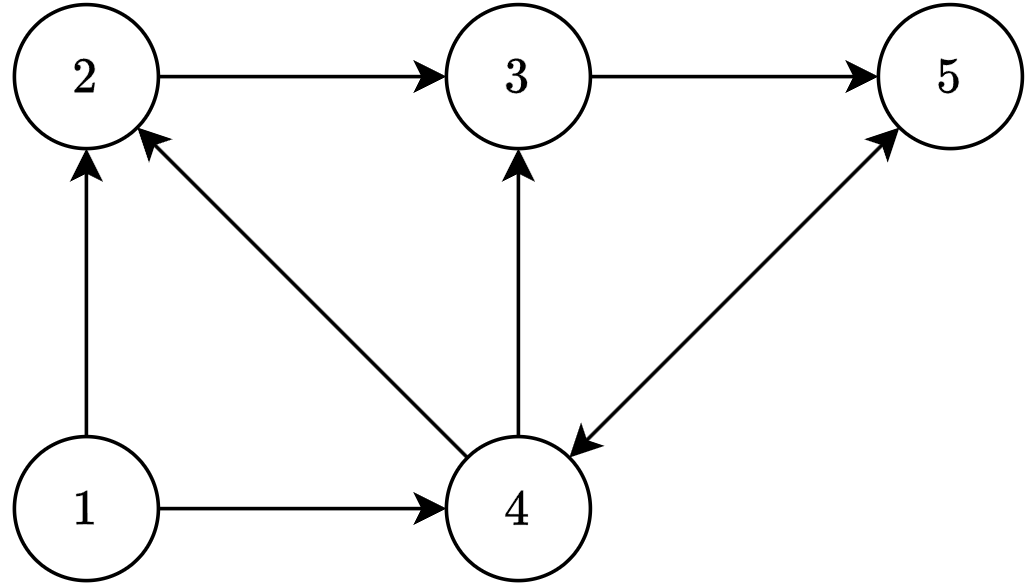
\includegraphics[width=0.3\linewidth]{images/graphs.png}
    \end{figure}
\end{example}